%%%%%%%%%%%%%%%%%%%%%%%%%%%%%%%%%%%%%%%%%%%%%%%%%%%%%%%%%%%%%%%%%%%%%%%%%%%%%
%
% File:   week1.tex
% Date:   06-Sep-2017
% Author: I. Chuang <ichuang@mit.edu>
%
% 2017 8.370 week 1
%

%\documentclass{article}
%\usepackage{graphicx}

\newcommand{\be}{\begin{equation}}
\newcommand{\ee}{\end{equation}}

\newcommand{\bea}{\begin{eqnarray}}
\newcommand{\eea}{\end{eqnarray}}

%Ryuji added
\usepackage{amsmath}
\newcommand{\ket}[1]{|{#1}\rangle}
\newcommand{\bra}[1]{\langle{#1}|}
\newcommand{\braket}[2]{\langle{#1}|{#2}\rangle}
\newcommand{\ketbra}[2]{|{#1}\rangle\!\langle{#2}|}
%%%%%%%%%%%%%%%%%%%%%%%%%%%%%%%%%%%%%%%%%%%%%%%%%%%%%%%%%%%%%%%%%%%%%%%%%%%%%
% problem environment (for PS)

\newenvironment{problem}{\begin{enumerate}%
		\renewcommand{\makelabel}[1]{%
  		    {\bf \TheType\refstepcounter{mycnt}\themycnt:~\hfill}%
		    \ifthenelse{\equal{##1}{}}{}{%
    		({\bf ##1})}%
			}}%
                        {\end{enumerate}}%

\newcommand{\mattwoc}[4]{\left[
    % \setlength{\arraycolsep}{4pt}%
	\begin{array}{cc}{#1}&{#2}\\{#3}&{#4}\end{array}\right]}

%%%%%%%%%%%%%%%%%%%%%%%%%%%%%%%%%%%%%%%%%%%%%%%%%%%%%%%%%%%%%%%%%%%%%%%%%%%%%
% Main Text

\def\<{\langle}
\def\>{\rangle}

\begin{edXchapter}{Unit 1: Quantum and classical computing fundamentals}[url_name=unit1]

\edXaskta{settings=1 to=rtakagi@mit.edu cc=ichuang@mit.edu}

% 
%%%%%%%%%%%%%%%%%%%%%%%%%%%%%%%%%%%%%%%%%%%%%%%%%%%%%%%%%%%%%%%%%%%%%%%%%%%%%

\begin{edXsection}{Introduction to 8.370r}

\begin{edXtext}{About this course}

{\LARGE About this course}

{\noindent\bf\Large Welcome to 8.370r Quantum Information Science I.}

This course rovides an introduction to the theory and practice of quantum
computation. We cover the physics of information processing;
quantum logic; quantum algorithms including Shor's factoring algorithm
and Grover's search algorithm; quantum error correction; quantum
communication and cryptography. Prior knowledge of quantum mechanics
helpful but not required. This is the first course in a sequence of two
quantum information science courses at MIT.

You may find helpful the
\href{https://www.edx.org/course/mastering-quantum-mechanics-part-1-wave-mitx-8-05-1x}{MIT
  8.05x courses on edX}, and Berkeley's
\href{https://www.edx.org/course/quantum-mechanics-quantum-computation-uc-berkeleyx-cs-191x}{CS191
  course}.  The
\href{https://www.edx.org/course/quantum-cryptography-caltechx-delftx-qucryptox}{Caltech-TU
  Delft course on quantum cryptography} may also be insightful.

This course comprises four units, each with lectures and
in-depth, automatically graded problems:
\begin{itemize}
\item{\href{/course/courseware/unit1}{Unit 1: Quantum and classical
    computing fundamentals}} -- an introduction to quantum computation;
  classical Boolean logic; introduction to quantum mechanics; and
  quantum wierdness.

\item{\href{/course/courseware/unit2}{Unit 2: Simple quantum protocols
    and algorithms}} -- covering quantum teleportation, superdense
  coding, the quantum circuit model, the Deutsch-Jozsa quantum
  algorithm, Simon's algorithm, the quantum Fourier transform, phase
  estimation, and Shor's quantum factoring algorith.

\item{\href{/course/courseware/unit3}{Unit 3: Quantum noise, codes,
    and communication}} -- illustrating classical error correction
  codes, quantum noise models, the nine-qubit quantum code, criteria
  for quantum codes, Calderbank-Shor-Steane codes, and quantum key
  distribution.

\item{\href{/course/courseware/unit4}{Unit 4: Models of quantum
    computation}} -- describing the role of measurement in quantum
  algorithms, distributed quantum algorithms, noisy computation and
  fault-tolerance, quantum fault-tolerance, and adiabatic quantum
  computation.

\end{itemize}

{\noindent\bf\Large Assessments and Deadlines}

There are eight problem sets - two for each unit.  

{\noindent\bf\Large Grading and Certificates}

The course grade is 40\% homework, 20\% midterm exam, 30\% final exam, and 10\% participation.

{\noindent\bf\Large Honor Code}

As described in the \href{https://www.edx.org/edx-terms-service}{edX Honor code}, you are expected to:

\begin{itemize}
  \item
    Complete all tests and assignments on my own, unless collaboration on an assignment is explicitly permitted.
  \item
    Maintain only one user account and not let anyone else use my username and/or password.
  \item
    Not engage in any activity that would dishonestly improve my results, or improve or hurt the results of others.
  \item
    Not post answers to problems that are being used to assess student performance.
\end{itemize}

{\noindent\bf\Large Textbook and References}

You may find it helpful to refer to:
\href{https://www.amazon.com/Quantum-Computation-Information-10th-Anniversary/dp/1107002176}{Quantum
  Computation and Quantum Information}, by Nielsen and Chuang.  There are also excellent, freely available 
\href{http://www.theory.caltech.edu/~preskill/ph219/index.html#lecture}{lecture notes by John Preskill}, and 
superb \href{http://pirsa.org/C15009}{video lectures by Daniel Gottesman}.

% \edXaskta{settings=1 to=csamolis@mit.edu cc=ichuang@mit.edu}

\end{edXtext}

\end{edXsection}

%%%%%%%%%%%%%%%%%%%%%%%%%%%%%%%%%%%%%%%%%%%%%%%%%%%%%%%%%%%%%%%%%%%%%%%%%%%%%


%%%%%%%%%%%%%%%%%%%%%%%%%%%%%%%%%%%%%%%%%%%%%%%%%%%%%%%%%%%%%%%%%%%%%%%%%%%%%

% \input{week1_1_survey.tex}

%%%%%%%%%%%%%%%%%%%%%%%%%%%%%%%%%%%%%%%%%%%%%%%%%%%%%%%%%%%%%%%%%%%%%%%%%%%%%

\begin{edXsection}{Lectures U1.1: History and development of quantum computation}

%%%%%%%%%%%%%%%%%%%%

\begin{edXvertical}{About Unit 1}

\begin{edXtext}{About Unit 1}

{\LARGE About Unit 1}

{\noindent\bf \underline{Lecture Topics:}} Introduction to quantum
computation; classical Boolean logic; introduction to quantum
mechanics; quantum wierdness.

We begin this course with an overview of quantum computation, then
build a foundation for the semester by describing the basic tenets of
classical computing, based on Boolean logic.  We then present the
fundamental principles of quantum mechanics, in the context of quantum
computation, based on four postulates governing states, time-evolution
of states, measurement, and tensor products of states.  We then
illustrate some of the strangest, non-classical features of quantum
mechanics, many of which arise in the context of a property known as
quantum entanglement.

~\\
{\noindent\bf \underline{Optional Reading:}}
\href{https://www.amazon.com/Quantum-Computation-Information-10th-Anniversary/dp/1107002176}{Nielsen and Chuang}, Chapter 1

% \edXaskta{settings=1 to=csamolis@mit.edu cc=ichuang@mit.edu}

\end{edXtext}

\AddSearchBox{1}

\end{edXvertical}

%%%%%%%%%%%%%%%%%%%%

\begin{edXvertical}{Course topics for the semester}

\edXvideo{Course topics for the semester}{mkEzEkrqrlk}[url_name=U1L1a]

\AddSearchBox{2}

\end{edXvertical}

%%%%%%%%%%%%%%%%%%%%

\begin{edXvertical}{Models for classical computation}

\edXvideo{Models for classical computation}{BM4hlDQsc1M}[url_name=U1L1b]

% \edXvideo{Density matrices}{37BFmLp8TTc}[url_name=Q1L2a]

\AddSearchBox{3}

\end{edXvertical}

%%%%

\begin{edXvertical}{CQ: Models for classical computation}

\begin{edXproblem}{Universality of classical circuits}{url_name=u1-1-cq-universality attempts=1}

This is a concept question, provided to double-check your understanding of the previous video clip.

In lecture, Prof. Shor introduced the topic of universality, and
described how some models of classical computation which are
universal, and other models are not.

The circuit model of classical computation may be defined as the
family of electrical circuits composed from AND gates and NOT gates.

Check all the following which are true for the circuit model:

\edXabox{type="oldmultichoice"
    expect="Circuits are universal for classical computation","Circuits can describe computations which are beyond what a Turing machine can do","Circuits can simulate Turing machines"
    options="Circuits are universal for classical computation","Circuits are NOT a universal model for classical computation","Circuits can describe computations which are beyond what a Turing machine can do","Circuits can simulate Turing machines"
}

\end{edXproblem}

\AddSearchBox{1}

\end{edXvertical}

%%%%%%%%%%%%%%%%%%%%

\begin{edXvertical}{History of quantum mechanics and quantum computation}

\edXvideo{History of quantum mechanics and quantum computation}{Fm{-}gIjGlpBo}[url_name=U1L1c]

\AddSearchBox{4}

\end{edXvertical}

%%%%

\begin{edXvertical}{CQ: Faster-than-light communication with entanglement?}

\begin{edXproblem}{Faster-than-light communication with entanglement?}{url_name=u1-1-cq-qm-flash attempts=1}

This is a concept question, provided to double-check your understanding of the previous video clip.

As described by Prof. Shor in the last lecture video clip, in 1982,
Nick Herbert published
\href{https://link.springer.com/article/10.1007\%2FBF00729622}{a paper
  proposing FLASH}, ``First Laser-Amplified Superluminal Hookup,''
offering a means to communicate faster than the speed of light, using
quantum entanglement.

What was the flaw in Herbert's proposal?

\edXabox{type="multichoice"
    expect="Unknown quantum states cannot be copied"
    options="Entangled states have too short of a lifetime to allow superluminal communication","Entangled photons are states of light which cannot travel faster than the speed of light","Quantum entanglement involves hidden variables, which obfuscate any superluminal communication","Unknown quantum states cannot be copied"
}

\end{edXproblem}

\AddSearchBox{5}

\end{edXvertical}

%%%%%%%%%%%%%%%%%%%%

\begin{edXvertical}{Computation must be robust against noise}

\edXvideo{Computation must be robust against noise}{OFWyhxzLN7k}[url_name=U1L1d]

\AddSearchBox{6}

\end{edXvertical}

%%%%

\begin{edXvertical}{CQ: Mechanisms for fault-tolerance}

\begin{edXproblem}{Mechanisms for fault-tolerance}{url_name=u1-1-cq-qm-flash attempts=1}

This is a concept question, provided to double-check your understanding of the previous video clip.

Which of the following are mechanisms for fault-tolerance, as used in classical computing?  Check all which apply:

\edXabox{type="oldmultichoice"
    expect="Massive redundancy","Checkpointing","Error correction"
    options="Massive redundancy","Checkpointing","Code rewriting","Error correction"
}

\end{edXproblem}

\AddSearchBox{7}

\end{edXvertical}

%%%%%%%%%%%%%%%%%%%%

\end{edXsection}


%%%%%%%%%%%%%%%%%%%%%%%%%%%%%%%%%%%%%%%%%%%%%%%%%%%%%%%%%%%%%%%%%%%%%%%%%%%%%

\begin{edXsection}{PS#1 Part A - Reversible Circuits}

\begin{edXvertical}{Reversible two-four-three swap}

\begin{edXtext}{Classical Reversible Boolean Circuits}

{\LARGE Classical Reversible Boolean Circuits}

The following problems consitute the first part of PS\#1, and are due Thursday 14-Sep-2017 at 7pm ET.

The problems explore the construction of several useful reversible
circuits, using primitive reversible gates.

For each problem, please enter a text description of the gates to
apply, with one gate per line.  Allowed gates include NOT, \href{https://en.wikipedia.org/wiki/Controlled_NOT_gate}{CNOT},
\href{https://en.wikipedia.org/wiki/Toffoli_gate}{Toffoli}, and
\href{https://en.wikipedia.org/wiki/Fredkin_gate}{Fredkin} gates.
These are some examples of how you can specify gates and which bits
they act upon: \\

\begin{center}
  \begin{tabular}{cl}
    {\tt not(a)} & {NOT on a}  \\
{\tt cnot(a,b)} & {CNOT with control a and target b}   \\
{\tt swap(c,d)} & {swap on c,d}   \\
{\tt fredkin(a,b,c)} & {Fredkin with control a and targets b,c}   \\
{\tt toffoli(c,a,b)} & {Toffoli with controls c,a and target b}   \\
  \end{tabular}
\end{center}

These correspond to the following schematic drawing of the gates:
\centerline{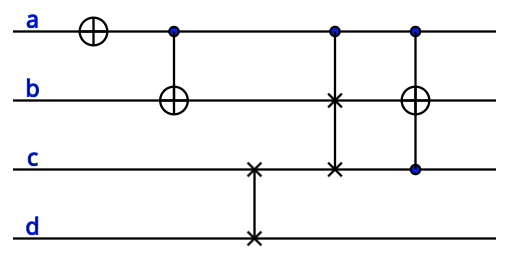
\includegraphics[width=500px]{figures/fig_reversible_gates.png}}

\end{edXtext}

%%%%%%%%%%%%%%%%%%%%%%%%%%%%%%%%%%%%%%%%

\begin{edXproblem}{Reversible two-four-three swap}{url_name=u1_1_four_input_cswap attempts=20}

\edXincludepy{lib/ftdigital2.py}

Design a reversible circuit, using NOT, CNOT, Toffoli, and Fredkin gates, which acts on the four inputs $a, b, c, d$, to perform the operation
${\rm swap_{243}}(a,b,c,d)$ which swaps $b$ and $d$ if $a=0$, and swaps $c$ and $d$ if $a=1$.  Bit $a$ should be left unchanged.

Note that you have 20 attempts, so you have some leeway with syntax
mistakes.  Most later problems will just provide 10.  Work out your
circuits in your own notebook and check carefully before entering; do
not rely on random exploration to get the correct answer.

\edXabox{type="custom" 
  rows=8   
  expect=""
  cfn="check_243_swap" 
  % math=1 
  % inline="1"
}


\begin{edXsolution}

  One correct solution is:
\begin{verbatim}
fredkin(a,c,d)
not(a)
fredkin(a,b,d)
not(a)
\end{verbatim}

\centerline{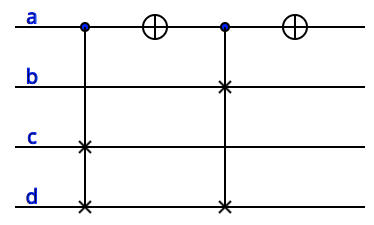
\includegraphics[width=500px]{figures/ps1a_swap243_circuit.png}}

\end{edXsolution}

\edXaskta{}

\end{edXproblem}

\AddSearchBox{001100}


\end{edXvertical}

%%%%%%%%%%%%%%%%%%%%%%%%%%%%%%%%%%%%%%%%

\begin{edXvertical}{Controlled-controlled swap}

\begin{edXproblem}{Controlled-controlled swap}{url_name=u1_1_ccswap attempts=10}

\edXincludepy{lib/ftdigital2.py}

Design a reversible circuit, using NOT, CNOT, Toffoli, and Fredkin gates, which acts on the four inputs $a, b, c, d$, to swap $c$ and $d$ only when both $a=1$ and $b=1$.  You may use a fifth bit $e$, given as initialized to $e=0$, in your circuit; this bit must also end as $e=0$.

\edXabox{type="custom" 
  % size=70   
  rows=8   
  expect=""
  cfn="check_ccswap" 
  % math=1 
  % inline="1"
}


\begin{edXsolution}

  One correct solution is:

\begin{verbatim}
fredkin(a,b,e)
fredkin(e,c,d)
fredkin(a,b,e)
\end{verbatim}

\centerline{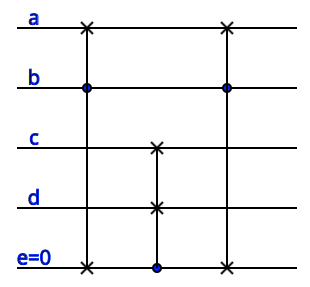
\includegraphics[width=500px]{figures/ps1a_ccswap_circuit.png}}

\end{edXsolution}

\edXaskta{}

\end{edXproblem}

\AddSearchBox{001101}

\end{edXvertical}

%%%%%%%%%%%%%%%%%%%%%%%%%%%%%%%%%%%%%%%%

\begin{edXvertical}{Reversible two-input demultiplexer}

\begin{edXproblem}{Reversible two-input demultiplexer}{url_name=u1_1_demux2 attempts=10}

\edXincludepy{lib/ftdigital2.py}

Design a reversible circuit, using NOT, CNOT, Toffoli, and Fredkin
gates, which acts on the two arbitrary inputs $a, b$, and the two
fixed inputs $c=0$, $d=0$, to produce four bits $a'$, $b'$, $c'$, $d'$
of output, where only the $n^{\rm th}$ output is $1$
(the others are all $0$), and $n=2b + a$.

This is a two-input demultiplexer, and the output is a unary encoded
value, sometimes otherwise known as \href{https://en.wikipedia.org/wiki/One-hot}{``one-hot encoding''} in the field
of deep neural networks.

\begin{edXshowhide}{Hint}
Denoting the NOT of $a$ as $\bar{a}$, note that
\bea
  a' &=& \bar{a} \bar{b} \\
  b' &=& a\bar{b} \\
  c' &=& \bar{a}b \\
  d' &=& ab
\,.
\eea

Since these are all Boolean functions of the input, it would seem
immediate how to compute these using Boolean logic functions.  The
trick here is that you're being asked to construct the circuit using
reversible gates, consuming no additional inputs, and producing no
extra garbage.  This is known as an ``in-place'' reversible circuit.

You should be able to do this using 11 gates.  If you can do it with fewer, let the TA know!
\end{edXshowhide}

\edXabox{type="custom" 
  % size=70   
  rows=8   
  expect=""
  cfn="check_demux2" 
  % math=1 
  % inline="1"
}

\begin{edXsolution}
  A reasonable solution is:

\begin{verbatim}
		toffoli(a,b,d)
		not(a)
                toffoli(a,b,c)
                not(a)
                cnot(d,b)
                cnot(c,b)
                not(d)
                toffoli(a,d,b)
                not(d)
                not(a)
                cnot(c,a)
\end{verbatim}

\centerline{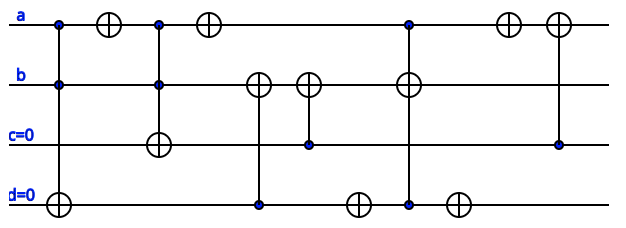
\includegraphics[width=500px]{figures/ps1a_demux2_circuit.png}}
  
\end{edXsolution}

\edXaskta{}

\end{edXproblem}

\AddSearchBox{001101}

\end{edXvertical}

%%%%%%%%%%%%%%%%%%%%%%%%%%%%%%%%%%%%%%%%
\end{edXsection}




%%%%%%%%%%%%%%%%%%%%%%%%%%%%%%%%%%%%%%%%%%%%%%%%%%%%%%%%%%%%%%%%%%%%%%%%%%%%%


\begin{edXsection}{PS#1 Part B - Quantum Mechanics}

\begin{edXvertical}{Pauli matrices}

\begin{edXproblem}{Eigenvalues, eigenstates}{attempts=20}

Recall from the linear algebra class that any normal linear operator $A$ (normal linear operator satisfies $AA^{\dagger}=A^{\dagger}A$) allows for a spectral decomposition
$A=\sum_i a_i \ketbra{i}{i}$ where $a_i$ is called eigenvalue and $\ket{i}$ is called eigenvector or eigenstate when $A$ is Hermitian. 

The Pauli matrices with $Z$ basis are 
\begin{equation}
 I=
 \begin{pmatrix}
  1 & 0\\
  0& 1 
 \end{pmatrix}
 ,
  X=
 \begin{pmatrix}
  0 & 1\\
  1& 0 
 \end{pmatrix}
 ,
  Y=
 \begin{pmatrix}
  0 & -i\\
  i& 0 
 \end{pmatrix}
 ,
  Z=
 \begin{pmatrix}
  1 & 0\\
  0& -1 
 \end{pmatrix}
\end{equation}

Compute the sets of eigenvalue and eigenstate for each Pauli matrix. Note that each Pauli matrix has a positive eigenvalue and a negative eigenvalue. Express the eigenstates with $Z$ basis ($\{\ket{0},\ket{1}\}$) using the ket notation. 

Type in \texttt{|0>} for $\ket{0}$ etc. and \texttt{sqrt(2)} for $\sqrt{2}$. For multiplication, do not forget to type \texttt{*}. For instance, you should type in \texttt{2*|0>} for $2\ket{0}$. You may use \texttt{i} for $i$.
  
% This is the line which pastes in the python code
\edXincludepy{lib/sympy_check.py}

$X$:
\edXinline{positive eigenvalue =} \edXabox{expect="1" type="numerical"
  tolerance='1\%' inline='1'},\ \edXinline{eigenstate =} \edXabox{expect="(|0>+|1>)/sqrt(2)" type="custom" cfn="sympy_check_quantum" inline='1' math="1"  preprocessorClassName="MathjaxPreprocessorForQM" preprocessorSrc="/static/mathjax_preprocessor_for_QM_H.js"}  

\edXinline{negative eigenvalue =} \edXabox{expect="-1" type="numerical"
  tolerance='1\%' inline='1' options=},\ \edXinline{eigenstate =} \edXabox{expect="(|0>-|1>)/sqrt(2)" type="custom" cfn="sympy_check_quantum" inline='1' math="1"  preprocessorClassName="MathjaxPreprocessorForQM" preprocessorSrc="/static/mathjax_preprocessor_for_QM_H.js"}  
  
$Y$:
\edXinline{positive eigenvalue =} \edXabox{expect="1" type="numerical"
  tolerance='1\%' inline='1' options=},\ \edXinline{eigenstate =} \edXabox{expect="(|0>+i*|1>)/sqrt(2)" type="custom" cfn="sympy_check_quantum" inline='1' math="1"  preprocessorClassName="MathjaxPreprocessorForQM" preprocessorSrc="/static/mathjax_preprocessor_for_QM_H.js"}

\edXinline{negative eigenvalue =} \edXabox{expect="-1" type="numerical"
  tolerance='1\%' inline='1' options=},\ \edXinline{eigenstate =} \edXabox{expect="(|0>-i*|1>)/sqrt(2)" type="custom" cfn="sympy_check_quantum" inline='1' math="1"  preprocessorClassName="MathjaxPreprocessorForQM" preprocessorSrc="/static/mathjax_preprocessor_for_QM_H.js"}  
  
$Z$:
\edXinline{positive eigenvalue =} \edXabox{expect="1" type="numerical"
  tolerance='1\%' inline='1' options=},\ \edXinline{eigenstate =} \edXabox{expect="|0>" type="custom" cfn="sympy_check_quantum" inline='1' math="1"  preprocessorClassName="MathjaxPreprocessorForQM" preprocessorSrc="/static/mathjax_preprocessor_for_QM_H.js"}

\edXinline{negative eigenvalue =} \edXabox{expect="-1" type="numerical"
  tolerance='1\%' inline='1' options=},\ \edXinline{eigenstate =} \edXabox{expect="|1>" type="custom" cfn="sympy_check_quantum" inline='1' math="1"  preprocessorClassName="MathjaxPreprocessorForQM" preprocessorSrc="/static/mathjax_preprocessor_for_QM_H.js"}  
  
  
\begin{edXsolution}

 All the Pauli matrices except $I$ have eigenvalues +1 and -1. Eigenvectors are in the row vector form,
 \begin{equation}
  X: \frac{1}{\sqrt{2}}(1,1) \mbox{ for eigenvalue +1}, \frac{1}{\sqrt{2}}(1,-1) \mbox{ for eigenvalue -1} 
 \end{equation}
 \begin{equation}
  Y: \frac{1}{\sqrt{2}}(1,i) \mbox{ for eigenvalue +1}, \frac{1}{\sqrt{2}}(1,-i) \mbox{ for eigenvalue -1} 
 \end{equation}
 \begin{equation}
  Z: (1,0) \mbox{ for eigenvalue +1}, (0,1) \mbox{ for eigenvalue -1} 
 \end{equation}
 Noting that $\ket{0}=(1,0)$ and $\ket{1}=(0,1)$ with $Z$ basis, the eigenstates in the ket notations are obtained.
 
\end{edXsolution}  

\edXaskta{}

\end{edXproblem}


\begin{edXproblem}{Basis changes}{attempts=10}
 Consider the unitary matrix
 \begin{equation}
   H=\frac{1}{\sqrt{2}}
 \begin{pmatrix}
  1 & 1\\
  1& -1 
 \end{pmatrix}.
 \end{equation}
  This important unitary is called Hadamard gate, which frequently appears in quantum circuits. 
  It is easy to check that the Hadamard gate converts $\ket{0}$ and $\ket{1}$ as
 \begin{equation}
  H\ket{0}=\frac{1}{\sqrt{2}}(\ket{0}+\ket{1}),\ \ H\ket{1}=\frac{1}{\sqrt{2}}(\ket{0}-\ket{1}).
 \end{equation} 
We define $\ket{+}=\frac{1}{\sqrt{2}}(\ket{0}+\ket{1})$ and $\ket{-}=\frac{1}{\sqrt{2}}(\ket{0}-\ket{1})$.
Express each Pauli matrix with $\{\ket{+},\ket{-}\}$ basis. Type in, for instance, \texttt{[[1,0],[0,1]]} for 
$\begin{pmatrix}
1 & 0\\
0 & 1
$.

% This is the line which pastes in the python code
\edXincludepy{lib/sympy_check.py}

$X$:
\edXabox{expect="[[1,0],[0,-1]]" type="custom" cfn="sympy_formula_check" inline='1' math="1" preprocessorClassName="MathjaxPreprocessorForQM" preprocessorSrc="/static/mathjax_preprocessor_for_QM_H.js"}

$Y$:
\edXabox{expect="[[0,i],[-i,0]]" type="custom" cfn="sympy_formula_check" inline='1' math="1" preprocessorClassName="MathjaxPreprocessorForQM" preprocessorSrc="/static/mathjax_preprocessor_for_QM_H.js"}

$Z$:
\edXabox{expect="[[0,1],[1,0]]" type="custom" cfn="sympy_formula_check" inline='1' math="1" preprocessorClassName="MathjaxPreprocessorForQM" preprocessorSrc="/static/mathjax_preprocessor_for_QM_H.js"}  

\begin{edXsolution}

 Using $\ket{+}=H\ket{0}$ and $\ket{-}=H\ket{1}$, 
 \begin{equation}
  \bra{+}X\ket{+}=\bra{0}HXH\ket{0}=\bra{0}Z\ket{0}=1,\ \bra{+}X\ket{-}=\bra{0}Z\ket{1}=0\\
  \bra{-}X\ket{+}=\bra{1}Z\ket{0}=0,\ \bra{-}X\ket{-}=\bra{1}Z\ket{1}=-1\\ 
 \end{equation}
 For the other two, use $HYH=-Y$, $HZH=X$.
\end{edXsolution}

\end{edXproblem}

\end{edXvertical}

%%%%%%%%%%%%%%%%%%%%%%%%%%%%%%%%%%%%%%%%%%%%

\begin{edXvertical}{Quantum gates}

\begin{edXproblem}{Quantum gates}{attempts=10}

Quantum gates are building blocks of quantum circuits that drive the evolution of quantum states. 
The Hadamard gate was already introduced in the previous problem. We introduce another important gate called phase gate defined by 
\begin{equation}
 S=
 \begin{pmatrix}
  1 & 0 \\
  0 & i 
 \end{pmatrix}
\end{equation}
If we take the Hermitian conjugate, we obtain
\begin{equation}
 S^{\dagger}=
 \begin{pmatrix}
  1 & 0 \\
  0 & -i 
 \end{pmatrix}
\end{equation}
The phase gate does not do anything to $\ket{0}$ but adds the phase $i$ to $\ket{1}$.
For instance, $S\ket{+}=\frac{1}{\sqrt{2}}(\ket{0}+i\ket{1})$.

Quantum gates can be sequentially applied and the effective operation to the quantum state is obtained by multiplying the matrices describing the quantum gates in order. 
For instance, if $X$ is applied first and $H$ follows it, the total operation is $HX$. 
Compute the following. 

% This is the line which pastes in the python code
\edXincludepy{lib/sympy_check.py}

\edXinline{$HX=$} \edXabox{expect="(1/sqrt(2))*[[1,1],[-1,1]]" type="custom" cfn="sympy_formula_check" inline='1' math="1" preprocessorClassName="MathjaxPreprocessorForQM" preprocessorSrc="/static/mathjax_preprocessor_for_QM_H.js"}

\edXinline{$SH=$} \edXabox{expect="(1/sqrt(2))*[[1,1],[i,-i]]" type="custom" cfn="sympy_formula_check" inline='1' math="1" preprocessorClassName="MathjaxPreprocessorForQM" preprocessorSrc="/static/mathjax_preprocessor_for_QM_H.js"}

\edXinline{$SXS^{\dagger}=$} \edXabox{expect="[[0,-i],[i,0]]" type="custom" cfn="sympy_formula_check" inline='1' math="1" preprocessorClassName="MathjaxPreprocessorForQM" preprocessorSrc="/static/mathjax_preprocessor_for_QM_H.js"}

\end{edXproblem}

\end{edXvertical}

%%%%%%%%%%%%%%%%%%%%%%%%%%%%%%%%%%%%%%

\begin{edXvertical}{Bloch sphere}

\begin{edXproblem}{Positions on the Bloch sphere}{attempts=10}

Any qubit state $\ket{\psi}$ can be expressed of the form
\begin{equation}
 \ket{\psi}=\cos\left(\frac{\theta}{2}\right)\ket{0}+e^{i\phi}\sin\left(\frac{\theta}{2}\right)\ket{1}
\end{equation}
up to global phases, and $(\theta, \phi)$ determines the position of the state on the Bloch sphere. Express the positions in terms of $(\theta, \phi)$ for the eigenstate corresponding to the ${\bf negative}$ eigenvalue of each non-identity Pauli matrix.
If $\phi$ is undetermined (could take any value), take $\phi=0$. Type in, for instance, \texttt{[pi,pi]} for $(\pi,\pi)$.

% This is the line which pastes in the python code
\edXincludepy{lib/sympy_check.py}

\edXinline{$X$:} \edXabox{type="custom" size=40 expect="[pi/2,pi]" noanswer=1 cfn="sympy_formula_check" inline="1" math="1" options="tolerance='0.01' "}

\edXinline{$Y$:} \edXabox{type="custom" size=40 expect="[pi/2,(3/2)*pi]" noanswer=1 cfn="sympy_formula_check" inline="1" math="1" options="tolerance='0.01' "}

\edXinline{$Z$:} \edXabox{type="custom" size=40 expect="[pi,0]" noanswer=1 cfn="sympy_formula_check" inline="1" math="1" options="tolerance='0.01' "}

\begin{edXsolution}

 Eigenvectors corresponding to the negative eigenvalue are
 \begin{equation}
  X:\ \ \frac{1}{\sqrt{2}}(\ket{0}-\ket{1}),\ \ (\theta,\phi)=(\pi/2,\pi)\\
  Y:\ \ \frac{1}{\sqrt{2}}(\ket{0}-i\ket{1}),\ \ (\theta,\phi)=(\pi/2,3\pi/2)\\
  Z:\ \ \ket{1},\ \ (\theta,\phi)=(\pi,\mbox{undertmined})
 \end{equation}
 
\end{edXsolution}

\end{edXproblem}

\begin{edXproblem}{Single qubit rotation}{attempts=10}

Any unitary matrix in $SU(2)$ can be written of the form
\begin{equation}
 U=e^{-i\frac{\theta}{2} \vec{n}\cdot \vec{\sigma}}=\cos\left(\frac{\theta}{2}\right)I - i\sin\left(\frac{\theta}{2}\right)\vec{n}\cdot \vec{\sigma}
\end{equation}
It is regarded as a rotational operation on the Bloch sphere where $\theta$ and $\vec{n}=(n_x,n_y,n_z)$ specify the rotation angle and the axis which which the rotation takes place. $\vec{n}$ is a unit vector satisfying $n_x^2+n_y^2+n_z^2=1$. Note that $\vec{n}\cdot \vec{\sigma}=n_x\sigma_x+n_y\sigma_y+n_z\sigma_z$. We take $n_x\geq 0$ and $0\leq \theta <2\pi$ without loss of generality.
Find $\vec{n}$ and $\theta$ for the following unitary matrices. Type in, for instance, \texttt{[0,0,1]} for $(0,0,1)$. You may use \texttt{sqrt(2)} for $\sqrt{2}$.

% This is the line which pastes in the python code
\edXincludepy{lib/sympy_check.py}

$X$: 
\edXinline{$\vec{n}=$}\edXabox{type="custom" size=40 expect="[1,0,0]" noanswer=1 cfn="sympy_formula_check" inline="1" math="1" options="tolerance='0.01' "}
\edXinline{$\theta=$}\edXabox{type="custom" size=40 expect="pi" noanswer=1 cfn="sympy_formula_check" inline="1" math="1" options="tolerance='0.01' "}

$H=\frac{1}{\sqrt{2}}
\begin{pmatrix}
 1 & 1\\
 1 & -1
\end{pmatrix}
$: 
\edXinline{$\vec{n}=$}\edXabox{type="custom" size=40 expect="[1/sqrt(2),0,1/sqrt(2)]" noanswer=1 cfn="sympy_formula_check" inline="1" math="1" options="tolerance='0.01' "}
\edXinline{$\theta=$}\edXabox{type="custom" size=40 expect="pi" noanswer=1 cfn="sympy_formula_check" inline="1" math="1" options="tolerance='0.01' "}

$S=
\begin{pmatrix}
 1 & 0\\
 0 & i
\end{pmatrix}$: 
\edXinline{$\vec{n}=$}\edXabox{type="custom" size=40 expect="[0,0,1]" noanswer=1 cfn="sympy_formula_check" inline="1" math="1" options="tolerance='0.01' "}
\edXinline{$\theta=$}\edXabox{type="custom" size=40 expect="pi/2" noanswer=1 cfn="sympy_formula_check" inline="1" math="1" options="tolerance='0.01' "}

$SH$: 
\edXinline{$\vec{n}=$}\edXabox{type="custom" size=40 expect="[1/sqrt(3),1/sqrt(3),1/sqrt(3)]" noanswer=1 cfn="sympy_formula_check" inline="1" math="1" options="tolerance='0.01' "}
\edXinline{$\theta=$}\edXabox{type="custom" size=40 expect="(4/3)*pi" noanswer=1 cfn="sympy_formula_check" inline="1" math="1" options="tolerance='0.01' "}

\begin{edXsolution}
 $U=e^{-i\frac{\theta}{2}\vec{n}\cdot \sigma}$ can be explicitly written as
 \begin{equation}
  U=\begin{pmatrix}
   \cos(\theta/2)-i\sin(\theta/2)n_z & -i\sin(\theta/2)n_x-\sin(\theta/2)n_y\\
   -i\sin(\theta/2)n_x+\sin(\theta/2)n_y & \cos(\theta/2)+i\sin(\theta/2)n_z 
  \end{pmatrix}
 \end{equation} 
 
 We will see the first one closely. All the others can be obtained in similar ways. 
 $X=\begin{pmatrix}
   0 & 1\\
   1 & 0
  \end{pmatrix}
  $\\
 $n_z=0$ because the diagonal entries are zero. Equating the real part and imaginary part of $(1,2)$ entry and $(2,1)$ entry gives $n_x=1,n_y=0$, and $\theta=\pi$. $\vec{n}=(1,0,0)$ and $\theta=\pi$ gives $U=-iX$. Since the global phase does not play any role, we do not have to worry about $-i$ part. We say that $U$ is equivalent to $X$ up to global phases. 
 
\end{edXsolution}

\end{edXproblem}

\begin{edXproblem}{Single qubit rotation}{attempts=10}

What are the resulting positions when the following unitaries are applied to the state positioned $(\pi/2, 0)$? Answer in terms of $(\theta, \phi)$. Take $\phi=0$ when $\phi$ is not determined (could take any value).

% This is the line which pastes in the python code
\edXincludepy{lib/sympy_check.py}

$X:$
\edXabox{type="custom" size=40 expect="[pi/2,0]" noanswer=1 cfn="sympy_formula_check" inline="1" math="1" options="tolerance='0.01' "}

$S:$
\edXabox{type="custom" size=40 expect="[pi/2,pi/2]" noanswer=1 cfn="sympy_formula_check" inline="1" math="1" options="tolerance='0.01' "}

$SH:$
\edXabox{type="custom" size=40 expect="[0,0]" noanswer=1 cfn="sympy_formula_check" inline="1" math="1" options="tolerance='0.01' "}

$SHSH:$
\edXabox{type="custom" size=40 expect="[pi/2,pi]" noanswer=1 cfn="sympy_formula_check" inline="1" math="1" options="tolerance='0.01' "}

See how these gates rotate quantum states on the Bloch sphere and especially permute the eigenstates of Pauli matrices. 
 
\begin{edXsolution}

 The state corresponding to $(\pi/2,0)$ is $\ket{+}=\frac{1}{2}(\ket{0}+\ket{1})$.
 Apply the unitaries to it and find $\theta$ and $\phi$ such that $U\ket{+}=\cos(\theta/2)+e^{i\phi}\sin(\theta/2)$. 
 
\end{edXsolution} 
 
\end{edXproblem}

\end{edXvertical}

%%%%%%%%%%%%%%%%%%%%%%%%%%%%%%%%%%%%%%%%%%%%%%

\end{edXsection}


% 
% \input{week1_3_osr.tex}
% 
% \input{week1_4_denmat.tex}
% 
% \input{week1_lectures2.tex}
% 
% \input{week1_5_qec.tex}
% 
% \input{week1_6_ibm.tex}

% \input{week1_6_research.tex}

%%%%%%%%%%%%%%%%%%%%%%%%%%%%%%%%%%%%%%%%%%%%%%%%%%%%%%%%%%%%%%%%%%%%%%%%%%%%%
\end{edXchapter}
